%initialisation 
\documentclass[10pt,a4paper]{article}


\usepackage[utf8]{inputenc}%encodage des caractères
\usepackage[T1]{fontenc}%encodage de la police
\usepackage[french]{babel}%langue française
\usepackage{hyperref}
\usepackage{amsmath}
\usepackage{graphicx}
\usepackage{multicol}
\usepackage{listingsutf8}
\usepackage{caption}
\usepackage[
  backend=biber, 
  citestyle=authortitle-comp
]{biblatex}
\addbibresource{bib/S0016003200000107.bib}
\bibliography{bib/S0016003200000107}
\usepackage{algpseudocode}

\usepackage[usenames, dvipsnames]{color}

\usepackage[utf8]{inputenc}
\frenchbsetup{StandardLists=true} % à inclure si on utilise \usepackage[french]{babel}
\usepackage{enumitem}
\usepackage{amssymb}

\newcounter{nalg}[section] % defines algorithm counter for chapter-level
\renewcommand{\thenalg}{\thesection .\arabic{nalg}} %defines appearance of the algorithm counter
\DeclareCaptionLabelFormat{algocaption}{Algorithm \thenalg} % defines a new caption label as Algorithm x.y

\lstnewenvironment{algorithm}[1][]
{   
    \refstepcounter{nalg} 
    \captionsetup{labelformat=algocaption,labelsep=colon}
    \lstset{ 
        mathescape=true,
        frame=tB,
        numbers=left, 
        numberstyle=\tiny,
        basicstyle=\scriptsize, 
        keywordstyle=\color{black}\bfseries\em,
        keywords={Retourner, Si, Tant que, Sinon, Ajouter, def, Racine } 
        numbers=left,
        escapeinside={\%*}{*)},
        #1
    }
}
{}



%_______Document_______

\begin{document}

\begin{titlepage}

%Logo unicaen
\begin{figure}[t]

\includegraphics[scale=0.15]{img/unicaen.jpg}
\raggedleft
\end{figure}

\Large{\framebox(350,100){\textbf{RAPPORT PROJET 2 }}}\\
\centering{Sujet : \textbf{Analyse des algorithmes de tris.}}

\begin{figure}[h]
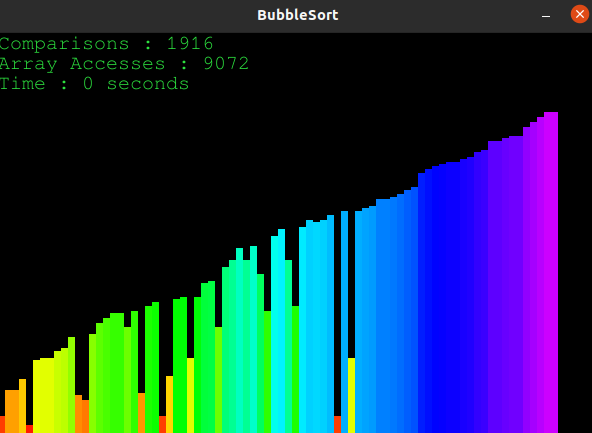
\includegraphics[scale=0.6]{img/view.png}
\caption{Visualisation de l'algorithme de tri BubbleSort.}
\label{fig:votre_image}
\centering
\end{figure}

\centering{ Nohan LEBRETON\\ Brian LONGUET \\ Harrisson KOBYLT \\ Oleg PAILLOT} \\
\centering{07/04/23}



%Supprime le numéro de page et l'initialise à 0.
\thispagestyle{empty}
\setcounter{page}{0}

\end{titlepage}

\section{Introduction}

    \subsection{Description générale du projet}
     Le tri de données est une opération fondamentale dans l'informatique, qui consiste à organiser un ensemble de données dans un ordre précis. Il existe de nombreux algorithmes de tri, chacun ayant ses avantages et ses inconvénients. Certains algorithmes sont plus efficaces que d'autres en fonction de la structure des données à trier, et certains peuvent même être optimisés en fonction de la distribution des données en entrée.\\

    L'objectif de ce projet est d'implémenter une collection d'algorithmes de tri et de les visualiser en action. Mais au-delà de cet aspect pratique, nous pouvons également nous intéresser à l'efficacité de ces algorithmes en fonction du niveau de désordre des données en entrée. En effet, le nombre de comparaisons, les accès aux données et le temps d'exécution total d'un algorithme peuvent varier considérablement en fonction de la quantité et de la répartition des données à trier.\\
    
    Pour répondre à cette question, nous devrons développer un générateur de données paramétré par un niveau de désordre, et effectuer des expériences pour comparer les performances des différents algorithmes de tri en fonction de ce paramètre. En analysant les résultats, nous pourrons déterminer quels algorithmes sont les plus adaptés à des situations de désordre élevé ou faible, et peut-être même proposer de nouvelles approches pour optimiser ces algorithmes en fonction des données en entrée.
    
    
\newpage
\subsection{Présentation du plan du rapport}
\tableofcontents
\newpage

\section{Objectifs du projet}
    \subsection{Problématique du projet}

    Comment est-ce que l'efficacité des algorithmes varie en fonction du degré de désordre des données, à savoir leur quantité et leur répartition ?
    
    \subsection{Description des points-clés et des grandes étapes}

        \begin{itemize}
            \item \textbf{Implémenter un générateur de tableau non trié permettant de spécifier un niveau de désordre (quantité et répartition)}: Nous avons implémenter un générateur de tableau non trié avec différents niveaux de désordre en utilisant l'entropie.
                
            L'entropie caractérise le degré de désorganisation, ou d'imprédictibilité, du contenu en information d'un système.
            
            \item \textbf{Implémenter autant d'algorithmes de tri que possible}: Nous avons implémenter les 11 algorithmes de tri suivants:
            
 
            \begin{multicols}{2}{
                \begin{itemize}  
                    \item \textbf{BubbleSort}
                    \item \textbf{CombSort}
                    \item \textbf{CountingSort}
                    \item \textbf{HeapSort}
                    \item \textbf{InsertionSort}
                    \item \textbf{MergeSort}
                \end{itemize} 
             
                \begin{itemize}  
                    \item \textbf{QuickSort}
                    \item \textbf{PancakeSort}
                    \item \textbf{SelectionSort}
                    \item \textbf{ShellSort}
                    \item \textbf{GnomeSort} 
                    \item \textbf{BogoSort}
                \end{itemize}
            }
            \end{multicols}

            \item \textbf{Implémenter le pattern strategy}: Nous avons implémenter le pattern strategy afin de définir la famille des algorithmes de tri.
            
            \item \textbf{Implémenter une visualisation des algorithmes de tri}: Nous avons implémenter une visualisation des algorithmes de tri à l'aide de la bibliothèque PyGame du langage de programmation Python.

            
            \item \textbf{Récupération des données de traitement des algorithmes de tri}:
            Nous avons redéfini des méthodes magiques de python afin d'obtenir les données suivantes: 
            
                \begin{itemize}  
                    \item \textbf{Temps(secondes)}
                    \item \textbf{Nombre de comparaisons} 
                    \item \textbf{Nombre d'accès au tableau}
                    \item \textbf{Nombre d'éléments}
                \end{itemize}
        

   
            \item \textbf{Expérimentations}: Nous avons mis en place des expérimentations afin d'obtenir les données nécessaires sur les algorithmes de tri pour réaliser une analyse des résultats.

            \item \textbf{Analyse des résultats}:Nous avons analysé les algorithmes selon les données du générateur de liste nous permettant ainsi de tirer une conclusion sur les différents algorithmes de tri.
            
        \end{itemize}

        
    \subsection{Description de travaux existants sur le même sujet}
     Nous nous sommes inspirés des travaux réalisés par d’autres développeurs sur le même thème, surtout du travail de Timo Bingman ‘The Sound of Sorting’. 
     Il a réalisé un logiciel de visualisation d’exécution de plusieurs algorithmes de tri en temps réel, il a également implémenté 15 algorithmes de tri. C’est grâce à son code réalisé en C++ que nous avons trouvé l’idée de créer des classes utilisant des "magic methods" pour compter automatiquement le nombre de comparaisons et d'accès au tableau d’un algorithme. Vous pouvez retrouver son projet sur son site  \href{https://panthema.net/}{panthema.net} .\\\\
     Il y a aussi le travail de Musiccombo ‘Array Visualize ’ qui nous a intéressé par son nombre impressionnant d’implémentations d’algorithmes. 



     
\section{Fonctionnalités implémentées}
    \subsection{Description des fonctionnalités}

        \subsubsection{Générateur de tableaux selon un niveau de désordre}
        L'entropie est, entre autre, une caractérisation du désordre dans un ensemble de valeurs. Notez cependant que ce désordre est lié aux valeurs et non à la répartition, ce n'est qu'une autre façon de voir le désordre dans un tableau. 

        \medskip
        L'implémentation du générateur que nous avons créé se base sur un algorithme mathématique existant\footcite{SWASZEK200097}. Nous avons pu le réécrire en code Python afin de pouvoir l'utiliser dans nos algorithmes de tri. Le pseudocode est visible en dessous.

        \pagebreak

        \begin{algorithm}[caption={Integer division.}, label={alg1}]
def gen_entropy(entropy,length)
    def entropy_minus_one(ent,q):
        x = ent - ((-q * log2(q)) - ((1-q) * log2(1-q)))
        Retourner x/(1-q)

    liste_proba = []
    liste_q = []
    liste_bracket = []

    Si entropy > log2(length)
        Alors arr%*ê*)t de l'algo
    
    temp_ent = entropy
    index_q = 0

    Pour i de length %*à*) 2 avec pas de -1
        def entropy_log(q):
            Retourner entropy_minus_one(temp_ent, q) - log2(i-1)
        def entropy_normal(q):
            Retourner entropy_minus_one(temp_ent, q)

        Si temp_ent >= 1 et temp_ent <= log2(i-1)
            j = Nombre flottant al%*é*)atoire entre 2^(-temp_ent) et 1
            Tant que 1
                Si entropy_minus_one(temp_ent,j) <= log2(i-1)
                    j = Nombre flottant al%*é*)atoire entre j et 1
                Sinon
                    g = j
                    Fin Tant que
            
            a = Racine de la fonction entropy_log entre l'intervalle 2^(-temp_ent) et g

            Ajouter (0,a) %*à*) liste_bracket
            Ajouter Nombre flottant al%*é*)atoire entre 0 et a %*à*) liste_q

        Sinon si temp_ent > log2(i-1):
            j = Nombre flottant al%*é*)atoire entre 0 et 2^(-temp_ent)
            Tant que 1
                Si entropy_minus_one(temp_ent,j) <= log2(i-1)
                    j = Nombre flottant al%*é*)atoire entre 0 et j
                Sinon
                    g1 = j
                    Fin Tant que

            j = Nombre flottant al%*é*)atoire entre 2^(-temp_ent) et 1
            Tant que 1
                Si entropy_minus_one(temp_ent,j) <= log2(i-1)
                    j = Nombre flottant al%*é*)atoire entre 1 et j
                Sinon
                    g2 = j
                    Fin Tant que

            a = Racine de la fonction entropy_log entre l'intervalle g1 et 2^(-temp_ent)
            b = Racine de la fonction entropy_log entre l'intervalle 2^(-temp_ent) et g2

            Ajouter (a,b) %*à*) liste_bracket
            Ajouter Nombre flottant al%*é*)atoire entre a et b %*à*) liste_q

        Sinon si temp_ent < 1
            j = Nombre flottant al%*é*)atoire entre 0 et 2^(-temp_ent)
            Tant que 1
                Si entropy_minus_one(temp_ent,j) <= 0
                    j = Nombre flottant al%*é*)atoire entre 0 et j
                Sinon
                    g1 = j
                    Fin Tant que

            j = Nombre flottant al%*é*)atoire entre 2^(-temp_ent) et 1
            Tant que 1
                Si entropy_minus_one(temp_ent,j) <= 0
                    j = Nombre flottant al%*é*)atoire entre j et 1
                Sinon
                    g2 = j
                    Fin Tant que

            j = Nombre flottant al%*é*)atoire entre 2^(-temp_ent) et 1
            Tant que 1
                Si entropy_minus_one(temp_ent,j) <= log2(i-1)
                    j = Nombre flottant al%*é*)atoire entre j et 1
                Sinon
                    g3 = j
                    Fin Tant que

            a = Racine de la fonction entropy_log entre l'intervalle g1 et 2^(-temp_ent)
            b = Racine de la fonction entropy_log entre l'intervalle 2^(-temp_ent) et g2
            c = Racine de la fonction entropy_log entre l'intervalle 2^(-temp_ent) et g3

            Si Nombre entier al%*é*)atoire entre [1;3[ == 1
                Ajouter (0,a) %*à*) liste_bracket
                Ajouter Nombre flottant al%*é*)atoire entre 0 et a %*à*) liste_q
            Sinon
                Ajouter (b,c) %*à*) liste_bracket
                Ajouter Nombre flottant al%*é*)atoire entre b et c %*à*) liste_q
        
        Si length > 2
            temp_ent = entropy_minus_one(temp_ent,liste_q[index_q])
            index_q += 1

    dernier_ent = temp_ent

    def entropy_binary(q):
        Retourner -q*log2(q) - (1-q)*log2(1-q) - dernier_ent

    j = Nombre flottant al%*é*)atoire entre 0 et 0.5
    Tant que 1
        Si entropy_binary(j) >= 0
            j = Nombre flottant al%*é*)atoire entre 0 et j
        Sinon
            g1 = j
            Fin Tant que

    j = Nombre flottant al%*é*)atoire entre 0.5 et 1
    Tant que 1
        Si entropy_binary(j) >= 0
            j = Nombre flottant al%*é*)atoire entre j et 1
        Sinon
            g2 = j
            Fin Tant que

    Ajouter Nombre flottant al%*é*)atoire entre g1 et 0.5 %*à*) liste_q
    Ajouter Nombre flottant al%*é*)atoire entre 0.5 et g2 %*à*) liste_q

    x = 1
    Pour i allant de 0 %*à*) length-2
        list_proba[i] = liste_q[i]*x
        x = x - liste_p[i]
    liste_p[length-2] = liste_q[length-2]*x
    liste_p[length-1] = liste_q[length-1]*x

    Retourner liste_q
        \end{algorithm}

        

        
        \subsubsection{Interface graphique}
        Au début de notre projet nous avons décidé d'implémenter une interface graphique afin de pouvoir visualiser et comparer les différents algorithmes de tri.\\
        Pour la partie concernant le choix des options et les inputs, nous avons décidé d'utiliser Tkinter qui implémente directement ce genre de fonctionnalité avec par exemple "Checkbutton".\\
        Tandis que pour l'affichage de la simulation des algorithmes nous avons choisi pygame, une fois de plus pour des raisons de simplicité et d'affinité avec ce que nous cherchions à faire.\\
        C'est ici qu'intervient le fichier tkMain.py. Celui-ci permet d'ouvrir une interface graphique tkinter. \\ L'utilisateur peut choisir une taille de liste, une entropie et s'il le souhaite, une seed et une précision.\\
        Puis il peut décider d'appliquer ces variables sur un algorithme, ou plusieurs s'il souhaite les comparer.\\
        Le ou les algorithmes s'exécutent alors avec les paramètres choisis, et si l'utilisateur en a décidé ainsi, les graphes comparant les algorithmes sont affichés et/ou enregistrés.\\
        Ces graphes permettent de comparer le temps pris par les algorithmes, le nombre de comparaisons qu'ils ont effectués et leur nombre d'accès au tableau.\\
        L'utilisateur peut également décider d'enregistrer tous les graphes dans des fichiers, dont il peut choisir les noms, ou d'enregistrer individuellement les graphes qu'il souhaite via l'interface matplotlib.\\
        
      
        
        \begin{figure}[h]
            \caption{\scriptsize Exemple de graphes obtenus après l'utilisation de l'interface}
            \centering
            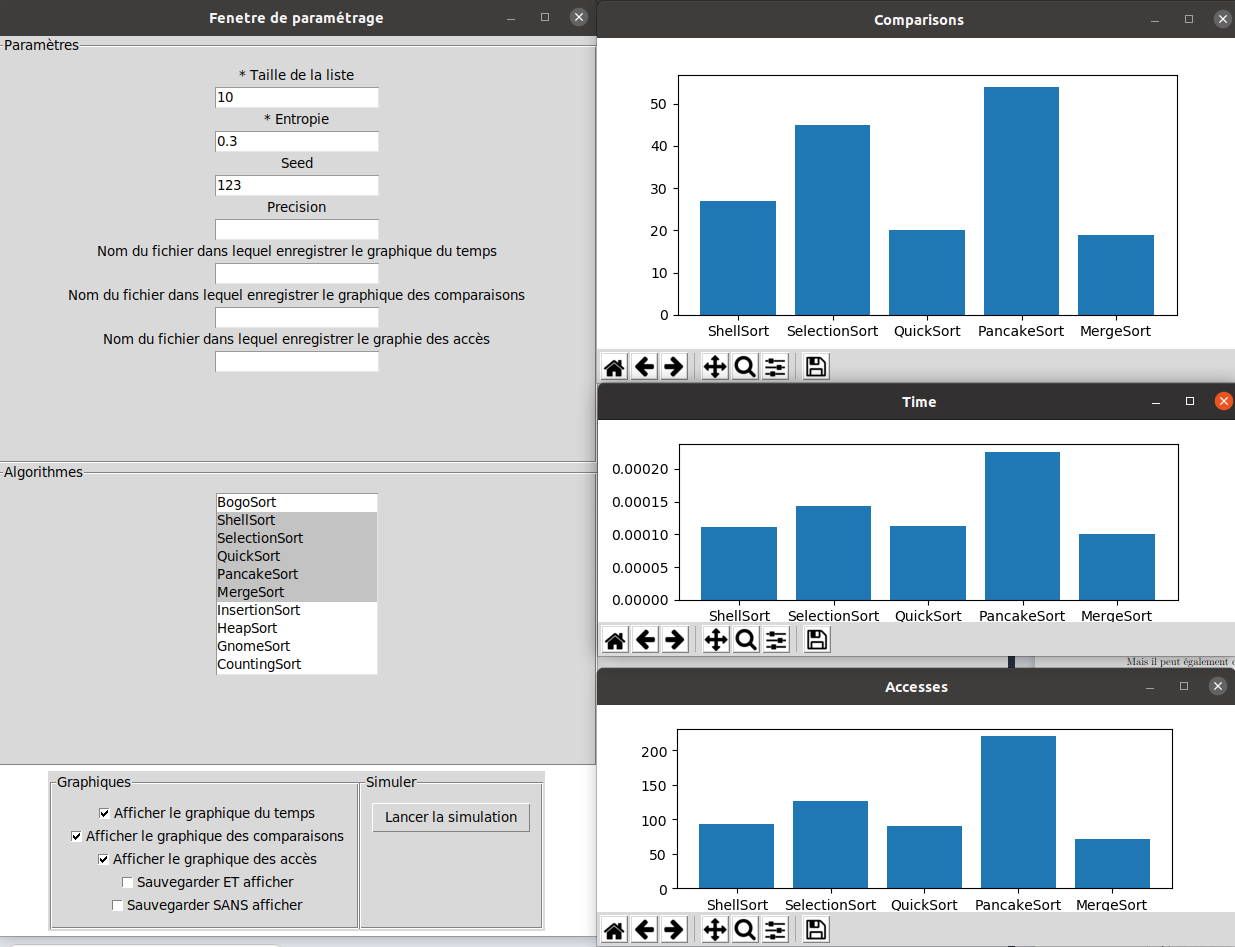
\includegraphics[scale=0.2]{img/interface.png}
        \end{figure}

        Quant à la simulation, que nous n'avons pas eu le temps de relier avec l'interface, celle-ci permet de visualiser en direct le tri d'une liste par un algorithme. Elle affiche également le nombre de comparaisons et d'accès tableau effectués, et le temps pris par l'algorithme afin de trier la liste.
                        
        En utilisant la visualisation faite à partir de PyGame, nous retrouvons les informations de base comme le nombre de comparaisons, d'accès au tableau ainsi que le temps d'exécution. Ici en plus nous avons le délai attribué entre chaque action (changement de couleur, remise à zéro de la couleur, swap, etc.), ainsi que le nombre de delai efféctués.
        
        \begin{figure}
            \caption{\scriptsize Exemple de visualisation PyGame avec l'algo BogoSort}
            \centering
            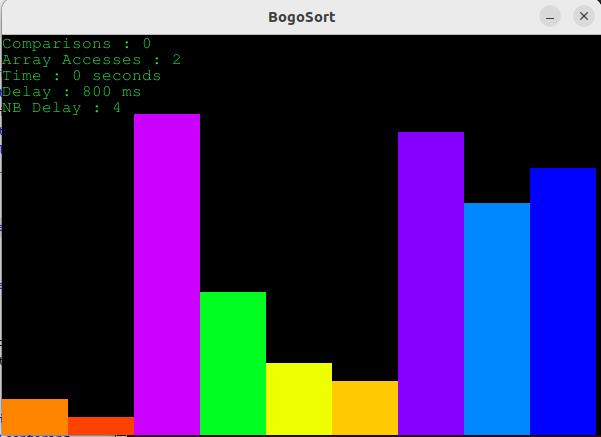
\includegraphics[scale=0.4]{img/pgVisual.png}
        \end{figure}
        
      \newpage

        
        
        \subsubsection{Tests unitaires}
        
            Nous avons choisi la mise en place de tests unitaires sur les deux parties les plus importantes à tester: le générateur d'entropie et les algorithmes de tri.

            
            \begin{figure}[h]
                \centering
                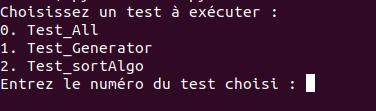
\includegraphics[scale=0.5]{img/test_runner.png}
            \end{figure}

            \begin{itemize}
                \item Tests sur le générateur d'entropie: on teste les différentes méthodes du générateur d'entropie.
                     \begin{figure}[h]
                    \centering
                    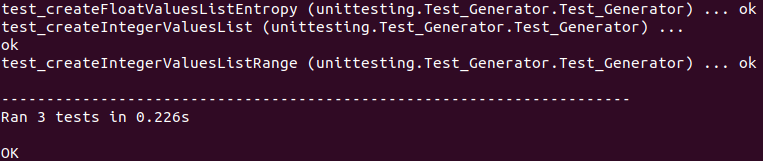
\includegraphics[scale=0.5]{img/test_generateur.png}
                \end{figure}
                
                \item Test sur les algorithmes de tri:
                on teste si les algorithmes implémentés retourne bien une liste trié.
                     \begin{figure}[h]
                    \centering
                    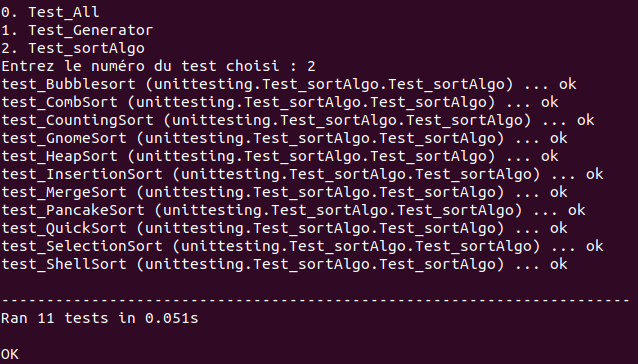
\includegraphics[scale=0.5]{img/test_algo.png}
                \end{figure}
            \end{itemize}
    


        
        \subsubsection{Scripts python et shell}
        Outre l'interface, il existe une autre façon d'exécuter les algorithmes; via des lignes de commande et des scripts.\\
        Dans un premier cas, via le fichier 'TERM.py', et la ligne de commande 'python3 TERM.py -a Algorithme -n tailleListe -e entropie -s seed -p precision', où :\\
         -a est le nom de l'algorithme a exécuter\\
         -n est la taille de la liste sur laquelle on souhaite exécuter l'algorithme\\
         -e est l'entropie que l'utilisateur souhaite appliquer a la liste\\
         -s la seed que l'utilisateur souhaite appliquer a la liste\\
         -p la précision appliquée aux nombres se trouvant dans la liste et les calculs\\
        qui exécute alors l'algorithme une fois. \\
        Dans un second cas, via le fichier 'termOPT.sh', et la ligne de commande './termOPT.sh -a Algorithme -n tailleListe -e entropie -s seed -p precision -i iteration -x cut', où : \\
         -i est le nombre de fois que l'on applique l'algorithme sur la liste donnée.\\
         -x cut permet de diviser la seed par le nombre d'itérations puis d'incrémenter celle-ci de manière régulière. \\
        Les résultats s'afficheront alors dans le terminal. \\
        Mais l'utilisateur peut également décider d'enregistrer les résultats dans un nouveau fichier en rajoutant ' > nomFichier.ExtensionFichier', ou à la suite d'un fichier déjà existant avec ' >> nomFichier.ExtensionFichier'\\
        TERM.py utilise la classe "ExecTri.py" qui permet d'exécuter les algorithmes ainsi que de récupérer le temps, le nombre d'accès au tableau et le nombre de comparaisons à l'aide de getters.\\
        Récupérer ces différents éléments nous permettent de compléter les graphes que nous créons dans l'interface décrite précédemment.\\

        
        \begin{figure}[h]
            \caption{\scriptsize Exemple de TERM.py lancé dans un terminal Linux.}
            \centering
            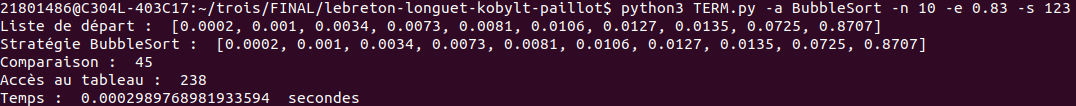
\includegraphics[scale=0.35]{img/TERM.png}
        \end{figure}
        

        \begin{figure}[h]
            \caption{\scriptsize Exemple de termOPT.sh lancé dans un terminal Linux.}
            \centering
            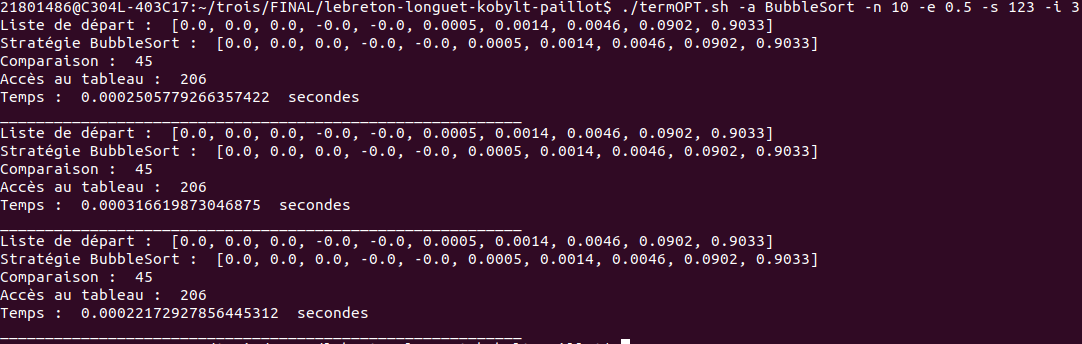
\includegraphics[scale=0.35]{img/termOPT.png}
        \end{figure}
        

        \newpage
         
        
    \section{Organisation du projet}
        Dès la première séance nous avons réussi à comprendre ce qui devait être effectué ( du moins dans les grandes lignes ), et à partir de cela, nous nous sommes départagés les tâches.\\
        Tout le monde a apporté beaucoup au projet avec un esprit d'équipe solide. Nous nous sommes aidés mutuellement à combler les lacunes de chacun pour que tout le monde soit au fait des différents travaux du groupe.
      
    \subsection{Trello et wiki de la forge unicaen}
    
        Nous avons opté pour l'utilisation de Trello afin d'organiser notre projet en découpant les différentes tâches en sous-tâches. Cela nous permet de nous entraider sur les points clés du projet grâce aux étiquettes, qui signalent avec des codes couleurs les sous-tâches urgentes, en cours, à faire, réalisées et les sous-tâches bonus.\\
        \textit{"Trello est un outil de gestion de projet en ligne, Il repose sur une organisation des projets en planches listant des cartes, chacune représentant des tâches. Les cartes sont assignables à des utilisateurs et sont mobiles d'une planche à l'autre, traduisant leur avancement."} Wikipédia.\\

        Notre lien Trello du projet: \href{https://trello.com/b/bvZ2Ye7e/projet2}{https://trello.com/b/bvZ2Ye7e/projet2}\\
        
        Nous avons également utilisé le wiki de la forge mis à disposition par l'université de Caen sur \href{https://forge.info.unicaen.fr}{forge.info.unicaen.fr}, afin que chacun puisse y accéder et y déposer des informations divers.
        
    \subsubsection{Nohan Lebreton}

       
                \begin{itemize}  
                    \item Implémentations d'algorithmes de tri
                    \item Réalisation des différents tests unitaires essentiels
                    \item Aide visualisation graphique notamment sur les pipes et le dégradé de couleur.
                    \item Préparation du rapport
                \end{itemize}
    
    \subsubsection{Oleg Paillot}
                \begin{itemize}  
                    \item Générateur d'entropie
                    \item Visualisation des résultats
                    \item Expérimentation
                \end{itemize}
    
    \subsubsection{Brian Longuet}
                \begin{itemize}  
                    \item Implémentions des algorithmes de tri
                    \item Visualisation graphique des algorithmes de tri
                \end{itemize}
    \subsubsection{Kobylt Harrisson}
                \begin{itemize}  
                    \item Interface graphique avec paramétrage et affichage de graphes et enregistrement de ceux-ci.
                    \item Scripts python et shell afin d'exécuter les algorithmes, afficher les résultats et enregistrer ceux-ci dans un fichier.
                \end{itemize}


        
    
         
        
    
\section{Éléments techniques}
    \subsection{Descriptions des algorithmes}
    \subsubsection{Algorithmes de tri implémentés}
     \begin{itemize}  
     
        \item SelectionSort: Ce tri sélectionne le plus petit élément et l'échange avec le premier élément. Puis, il sélectionne le deuxième plus petit élément et l'échange avec le deuxième élément, et ainsi de suite jusqu'à ce que la liste entière soit triée. C'est un algorithme simple mais inefficace pour les grandes listes.

        \item BubbleSort: Ce tri fonctionne en comparant deux éléments adjacents et en les échangeant s'ils ne sont pas dans le bon ordre. Il parcourt la liste plusieurs fois jusqu'à ce qu'il n'y ait plus d'échanges à faire, ce qui signifie que la liste est triée. C'est également un algorithme simple, mais pas très performant pour les grandes listes.
    
        \item InsertionSort: Ce tri prend chaque élément de la liste et l'insère à sa place appropriée dans la sous-liste triée qui le précède. Il est efficace pour les petites listes ou pour les listes partiellement triées.
    
        \item QuickSort: Ce tri utilise une stratégie de « diviser pour régner ». Il choisit un élément de la liste comme pivot, puis partitionne la liste en deux sous-listes, une avec les éléments plus petits que le pivot et une avec les éléments plus grands. Il répète ce processus récursivement jusqu'à ce que la liste soit triée. C'est l'un des tris les plus rapides pour les grandes listes.
    
        \item MergeSort: Ce tri utilise également une stratégie de « diviser pour régner ». Il divise la liste en deux sous-listes de taille égale (ou presque), les trie séparément, puis les fusionne pour former la liste triée. C'est également un algorithme rapide pour les grandes listes.
    
        \item HeapSort: Ce tri utilise une structure de données appelée tas (ou heap) pour trier les éléments. Il crée d'abord un tas à partir de la liste, puis répète l'extraction du plus grand élément du tas jusqu'à ce qu'il ne reste plus rien. C'est un algorithme efficace pour les grandes listes, mais il nécessite plus de mémoire que les autres algorithmes.
    
        \item CountingSort: Ce tri fonctionne en comptant le nombre d'occurrences de chaque élément distinct dans la liste, puis en utilisant ces comptages pour réorganiser la liste dans l'ordre trié. C'est un algorithme efficace pour les listes avec un petit nombre d'éléments distincts.
    
        \item ShellSort: Ce tri est une amélioration de l'InsertionSort. Il trie d'abord les éléments distants les uns des autres avec un certain intervalle, puis diminue progressivement cet intervalle jusqu'à ce qu'il atteigne 1 et effectue un tri par insertion standard. C'est un algorithme efficace pour les grandes listes.
    
        \item GnomeSort: Ce tri est similaire au BubbleSort, mais il utilise une approche différente pour les échanges d'éléments. Il parcourt la liste et compare chaque élément avec celui précédent. Si les éléments ne sont pas dans le bon ordre, il échange les deux éléments et recule d'un cran pour répéter la comparaison. C'est un algorithme simple mais inefficace pour les grandes listes.
    
        \item PancakeSort: Ce tri est un algorithme de tri qui consiste à inverser une partie de la liste à chaque étape pour la placer dans le bon ordre. À chaque étape, il trouve l'élément le plus grand et l'inverse avec le premier élément, puis il inverse toute la liste pour placer le plus grand élément à la fin de la liste triée. Il répète ce processus pour les sous-listes qui précèdent le plus grand élément jusqu'à ce que la liste entière soit triée. C'est un algorithme simple et intuitif, mais pas très efficace pour les grandes listes en raison du grand nombre d'inversions qu'il doit effectuer.

        \item CombSort: Ce tri est une amélioration de BubbleSort. Il utilise un facteur de réduction pour l'intervalle de comparaison des éléments, ce qui permet de comparer des éléments plus éloignés au fur et à mesure que la liste se rapproche d'un état trié. C'est un algorithme efficace pour les grandes listes et est souvent plus rapide que BubbleSort.

        \item BogoSort: Ce tri est un algorithme de tri aléatoire qui fonctionne en vérifiant si la liste est triée à chaque étape. S'il trouve que la liste n'est pas triée, il mélange aléatoirement la liste et répète le processus jusqu'à ce qu'il trouve une liste triée. C'est un algorithme très inefficace et imprévisible pour les grandes listes, mais il est utilisé parfois pour des listes de petites tailles à des fins pédagogiques.
    
      \end{itemize}
    
    \subsection{Descriptions des structures de données}

    Le générateur regroupe plusieurs méthodes, celle la plus intéréssante c'est la fonction "createFloatValuesListEntropy" qui retourne une liste contenant des nombres flottant où on a appliqué un certain pourcentage de désordre. 

    MonitoredList est une classe héritant de list, et permet grâce à ces "magic methods" redéfini d'incrémenter un compteur de d'accès au tableau. Utile pour connaître le nombre d'accès au tableau d'une algorithme. Possède également une méthode "getCompareCount" qui parcourt tous ces éléments de type FloatCompare et additionne leurs nombre de comparaison.

    FloatCompare est une classe héritant de float, et lorsqu'un algorithme fait une comparaison il incrémente le nombre de comparaison de l'élément comparé.

    
    
    \subsection{Description des données}
    Description des données : tu peux ici expliquer comment tu vas générer les données aléatoires avec différents niveaux de désordre.
    
\section{Architecture du projet}
    \subsection{Description des paquetages non standards utilisés}
    Description des paquetages non standards utilisés : si tu utilises des bibliothèques ou des modules externes pour ton projet, tu peux les présenter ici.

    Matplotlib nous l'utilisons pour générer des représentation graphique avec pour données les différents algorithmes de tri, ainsi que les comparaisons, les accès au tableau et le temps d'exécution.

    os nous l'utilisons surtout pour rajouter des arguments dans notre ligne de commande pour simplifier la vie de l'utilisateur. Verifier si un fichier est présent ou pas.

    Scipy nous l'utilisons dans le générateur, pour trouver une racine.

    Decimal utilisé aussi dans le générateur pour ne pas avoir de perte de précision.

    Numpy pour son module random générer une liste de nombre aléatoire.

    Math utilisé dans PipeFactory avec la fonction floor qui permet d'arrondie au dessus une valeur floatante. Utilisé également dans le générateur pour calculer les log.

    time pour obtenir le temps d'exécution d'un algorithme de tri.

    colorsys utilisé dans la classe Color qui converti des couleurs hsv en rgb pour réaliser le dégradé de couleur arc-en-ciel.

    pygame et tkinter permet d'afficher notre visualisation à l'écran, le menu pour rentrer les valeurs et l'affichage en temps réel l'exécution de l'algorithme.

    unittest permet de créer des tests unitaires.

    sys utilisé seulement dans la classe Window pour quitter proprement.

    ABC utilisé pour définir des classes abstraites dans les pattern observer et strategy.
    
    \subsection{Diagrammes des modules et des classes}
    Nous n'avons pas réussi a mettre le diagramme entier avec LaTex.
    La résolution du diagramme est bien trop grand, car nous l'avons générer avec pyreverse.
    Les digrammes se trouve dans le dossier diagramme de notre dossier rapport en LaTex.
    
    
    \subsection{Chaînes de traitement}
    Chaînes de traitement : tu peux ici expliquer comment les différents modules interagissent entre eux et comment les données sont traitées.
    
\section{Expérimentations}
    \subsection{Cas d’utilisation}

    Le plan d'expérimentation tourne autour d'un paramètre : l'entropie. Nous avons choisi une taille de liste fixe étant donné que notre but n'était pas de voir l'effet de la longueur du tableau à trier sur les algorithmes mais bien le désordre.\\

    L'entropie varie de 5 à 100\% avec un pas de 5\% pour chaque algorithme. La seed reste la même pour chaque algorithme.

    Nous prenons en sortie des expérimentations le temps d'exécution, le nombre d'accès à la liste de base et le nombre de comparaisons.
    
    \subsection{Résultats quantifiables}

    Vous pouvez voir les différents graphiques des expérimentations à la fin du rapport.
    
    \subsection{Analyse des résultats}
     Avec les graphiques, nous pouvons mettre en évidence une corrélation entre niveau de désordre et les différentes sorties des expérimentations pour certains des algos, mais pas tous.
     
\section{Conclusion}
    \subsection{Récapitulatif de la problématique et de la réalisation}
    Récapitulatif de la problématique et de la réalisation : tu peux ici résumer la problématique et ce que tu as fait pour y répondre.
    Nous avons grâce aux expérimentation une quantité de donnée sur le nombre de comparaisons, le nombre d'accès des données et le temps d'exécution sur les différents algorithmes implémenter en fonction de différentes entropie et une seed donnée. Nous pouvons donc réfléchir sur la problématique et comparer l'efficacité des algorithmes de tri.
 
    \subsection{Récapitulatif des résultats}
    Récapitulatif des résultats : tu peux ici résumer les résultats de tes expériences.

    \subsection{Propositions d’améliorations}

    \subsubsection{Interface graphique}
    \begin{itemize}
        \item Relier le bouton "lancer la simulation" avec la simulation créée par Brian
        \item Possibilité d'enregistrer l'ensemble des graphes dans un seul et même fichier ( au format .pdf par exemple ).
        \item Affichage du temps d'exécution d'un algorithme en temps réel et non après exécution complète ( dans la simulation ). 
        \item Ouverture d'une fenêtre indiquant lorsqu'une valeur est mal saisie ou lorsqu'une erreur se produit.
        \item L'utilisateur doit pouvoir choisir où il souhaite enregistrer les graphes créés. Dans le cas présent ils sont enregistrés dans le dossier où se trouve tkMain.py.
        \item Faire en sorte que la taille des graphes enregistrés change en fonction du nombre d'algorithmes présents dans le graphe. Afin que tout les noms soient visibles.
        \item Dans le meilleur des cas, avoir les mêmes options disponibles que dans le script "termOPT.sh".
    \end{itemize}
    
    \subsubsection{Scripts python et shell}
    \begin{itemize}
        \item Possibilité, lors de l'utilisation du script shell, de choisir quelles options parmi l'entropie, la seed et/ou la précision varient au cours du temps et à quelle "vitesse" ( en fonction d'un pas ). - En réalité, ça a été fait pour la seed, mais à cause d'une erreur de manipulation, le fichier a été supprimé et par manque de temps, il n'a pas pu être reproduit. 
        \item Dans le meilleur des cas, avoir les mêmes options disponibles que dans l'interface.
    \end{itemize}
    \subsubsection{Bonus}
    Parmi les idées que nous avons envisagées en tant que bonus, il y avait l'ajout d'un dégradé de couleur lors de la visualisation des algorithmes de tri avec l'interface graphique.
    Toutes les idées qui n'ont pas été mises en place en raison de leur manque de priorité incluent:
     \begin{itemize}  
        \item Visualisation en 3D: nous avons vue des projets similaire avec un visualisation en interface graphique des données a trier en 3D.
        \item Jeu pédagogique: il s'agit d'un jeu qui utilise l'interface graphique des algorithmes de tri à des fins pédagogiques. Le but est de deviner les différents algorithmes de tri simplement en observant leur visualisation graphique. 
        \item SortIA: il s'agit d'une IA qui apprend à partir de différents résultats et peut fournir le meilleur algorithme de tri pour une quantité et un désordre donnés.
        \item Ajout automatique des algorithmes : Faire en sorte que les algorithmes qui se trouvent dans le dossier approprié soient tous importés automatiquement. Cela permettrait de ne pas avoir a écrire/modifier chaque ligne d'import et cela permettrait à l'utilisateur d'ajouter ses propres algorithmes.
    \end{itemize}

\pagebreak
\printbibliography
\newpage

            \begin{figure}
                \centering
                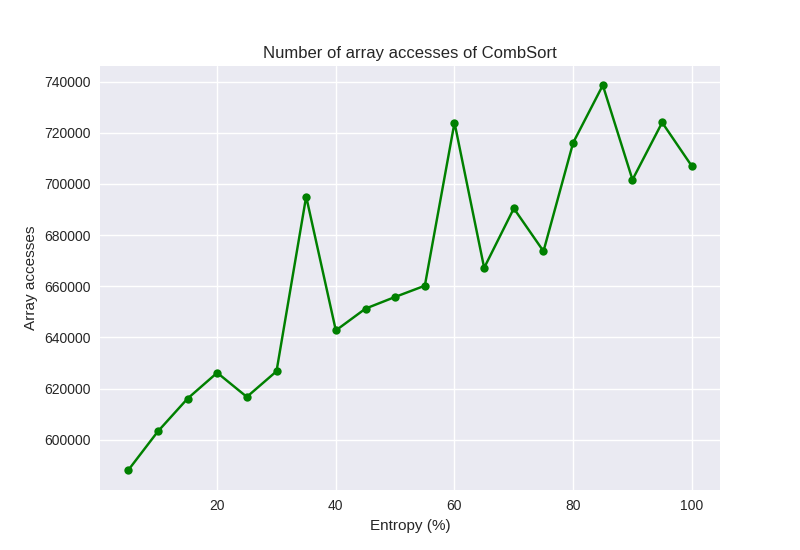
\includegraphics[width=1\textwidth]{graphique/CombSort/GraphAccessesCombSort.png}
                \caption{Graphique accès CombSort}
                \label{fig:mesh1}
            \end{figure}
            \begin{figure}
                \centering
                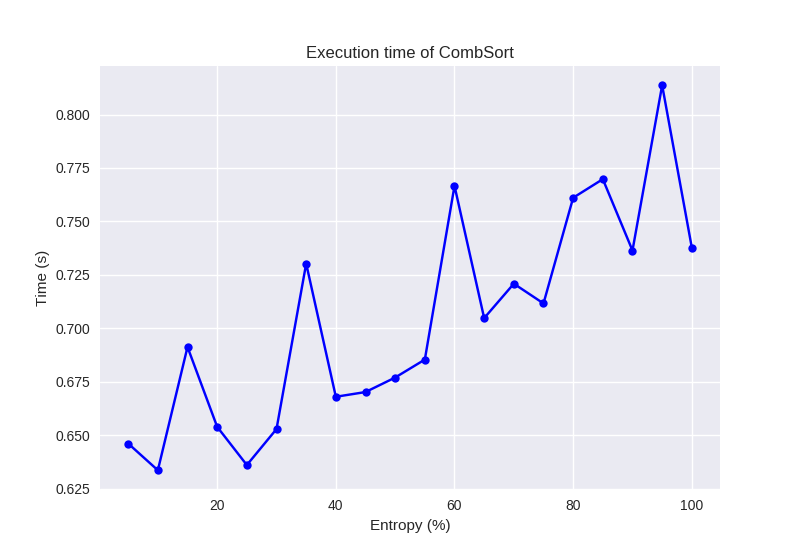
\includegraphics[width=1\textwidth]{graphique/CombSort/GraphTimeCombSort.png}
                \caption{Graphique temps CombSort}
                \label{fig:mesh1}
            \end{figure}
            \begin{figure}
                \centering
                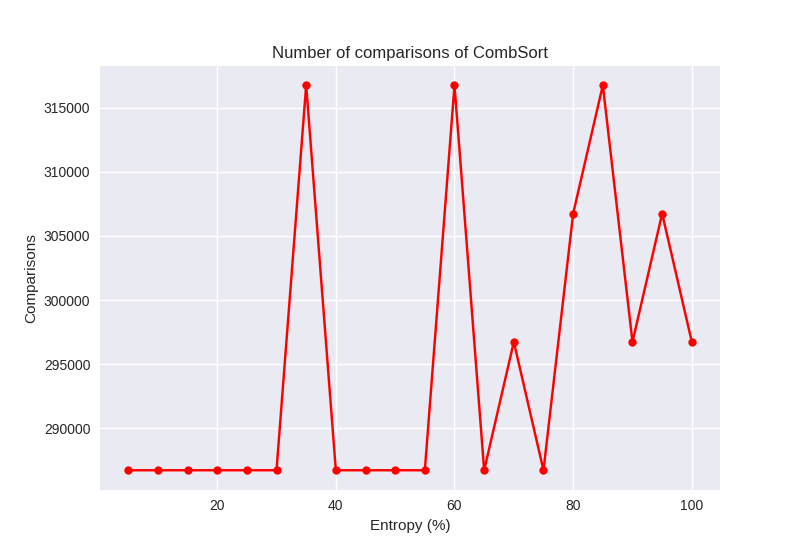
\includegraphics[width=1\textwidth]{graphique/CombSort/GraphComparisonsCombSort.png}
                \caption{Graphique comparaisons CombSort}
                \label{fig:mesh1}
            \end{figure}
%_________________________________________________
            \begin{figure}
                \centering
                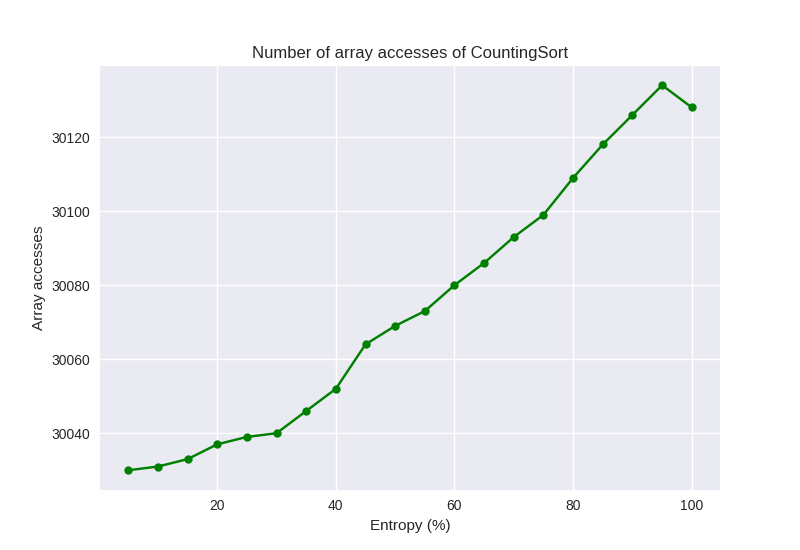
\includegraphics[width=1\textwidth]{graphique/CountingSort/GraphAccessesCountingSort.png}
                \caption{Graphique accès CountingSort}
                \label{fig:mesh1}
            \end{figure}
            \begin{figure}
                \centering
                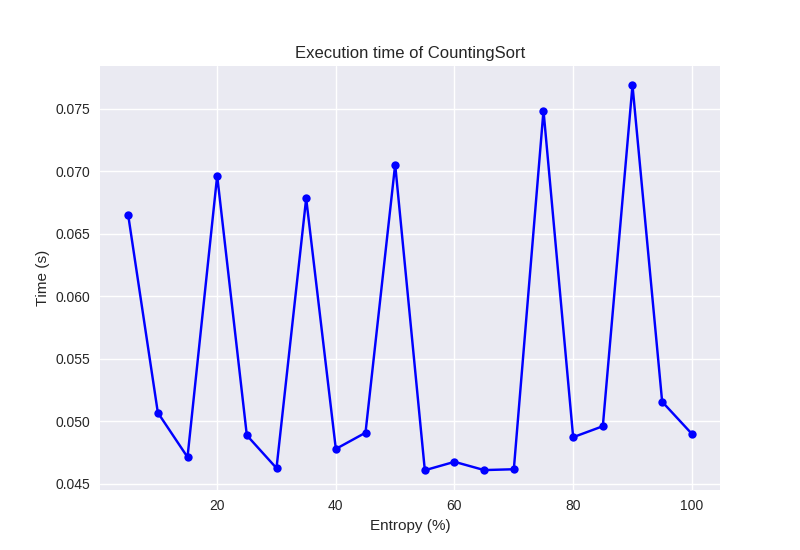
\includegraphics[width=1\textwidth]{graphique/CountingSort/GraphTimeCountingSort.png}
                \caption{Graphique temps CountingSort}
                \label{fig:mesh1}
            \end{figure}
            \begin{figure}
                \centering
                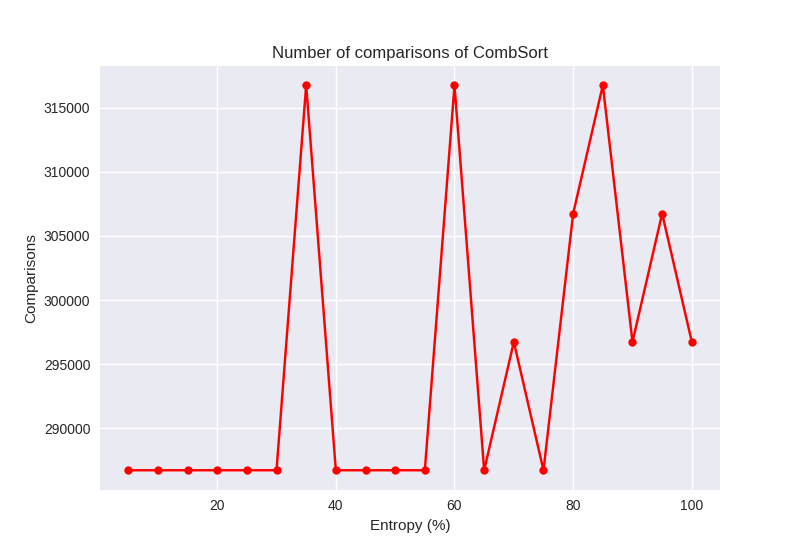
\includegraphics[width=1\textwidth]{graphique/CombSort/GraphComparisonsCombSort.png}
                \caption{Graphique comparaisons CountingSort}
                \label{fig:mesh1}
            \end{figure}
%_________________________________________________
            \begin{figure}
                \centering
                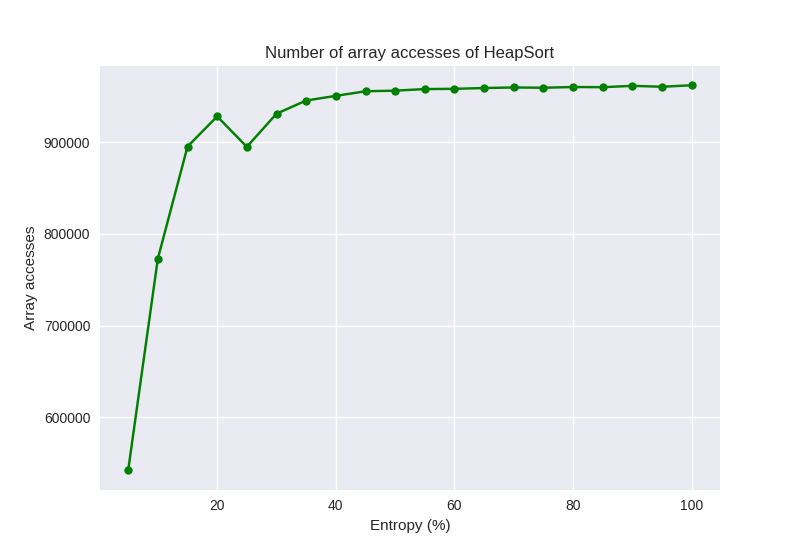
\includegraphics[width=1\textwidth]{graphique/HeapSort/GraphAccessesHeapSort.png}
                \caption{Graphique accès HeapSort}
                \label{fig:mesh1}
            \end{figure}
            \begin{figure}
                \centering
                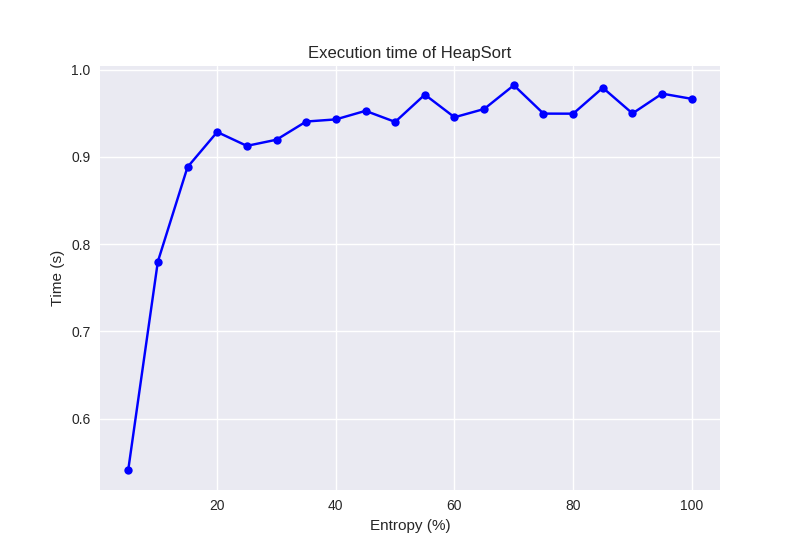
\includegraphics[width=1\textwidth]{graphique/HeapSort/GraphTimeHeapSort.png}
                \caption{Graphique temps HeapSort}
                \label{fig:mesh1}
            \end{figure}
            \begin{figure}
                \centering
                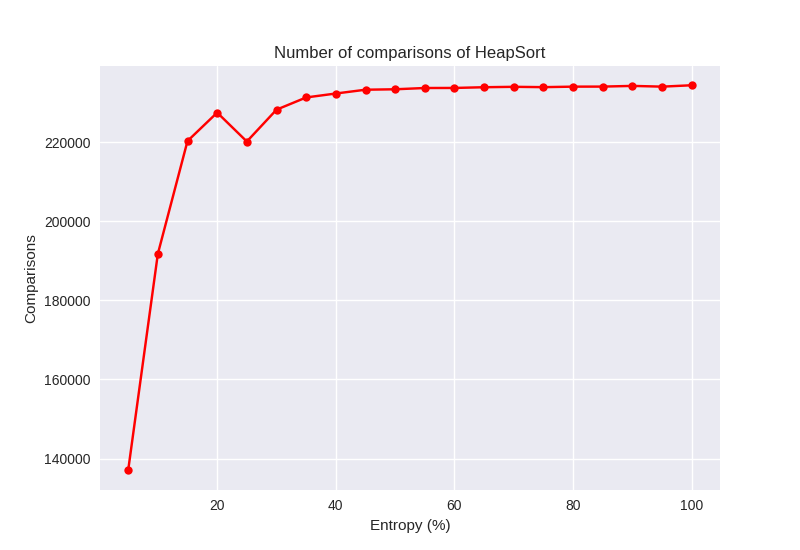
\includegraphics[width=1\textwidth]{graphique/HeapSort/GraphComparisonsHeapSort.png}
                \caption{Graphique comparaisons HeapSort}
                \label{fig:mesh1}
            \end{figure}

%_________________________________________________
            \begin{figure}
                \centering
                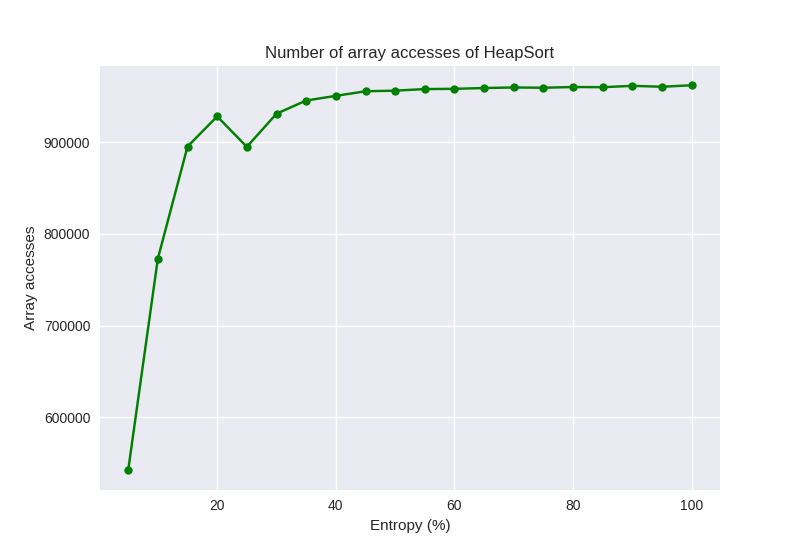
\includegraphics[width=1\textwidth]{graphique/HeapSort/GraphAccessesHeapSort.png}
                \caption{Graphique accès HeapSort}
                \label{fig:mesh1}
            \end{figure}
            \begin{figure}
                \centering
                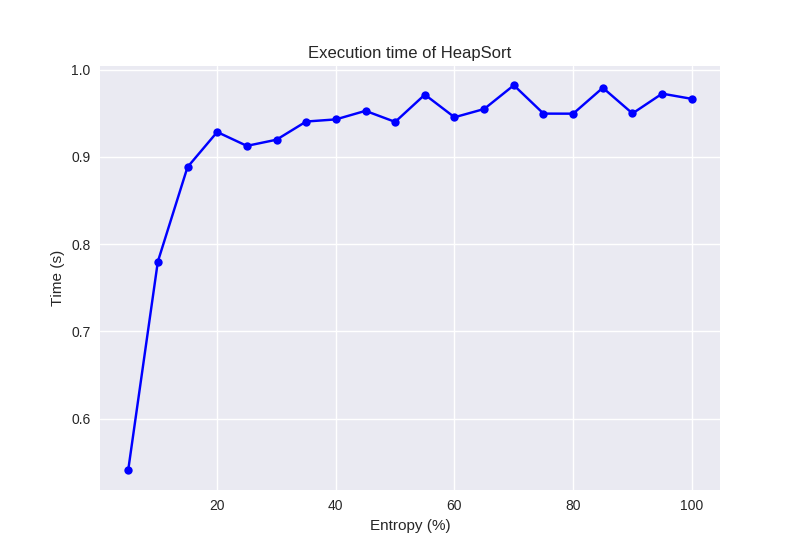
\includegraphics[width=1\textwidth]{graphique/HeapSort/GraphTimeHeapSort.png}
                \caption{Graphique temps HeapSort}
                \label{fig:mesh1}
            \end{figure}
            \begin{figure}
                \centering
                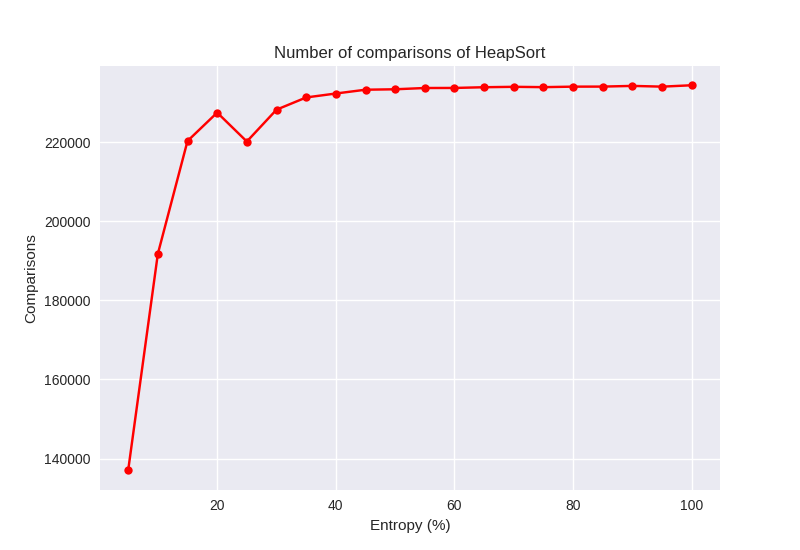
\includegraphics[width=1\textwidth]{graphique/HeapSort/GraphComparisonsHeapSort.png}
                \caption{Graphique comparaisons HeapSort}
                \label{fig:mesh1}
            \end{figure}

%_________________________________________________
            \begin{figure}
                \centering
                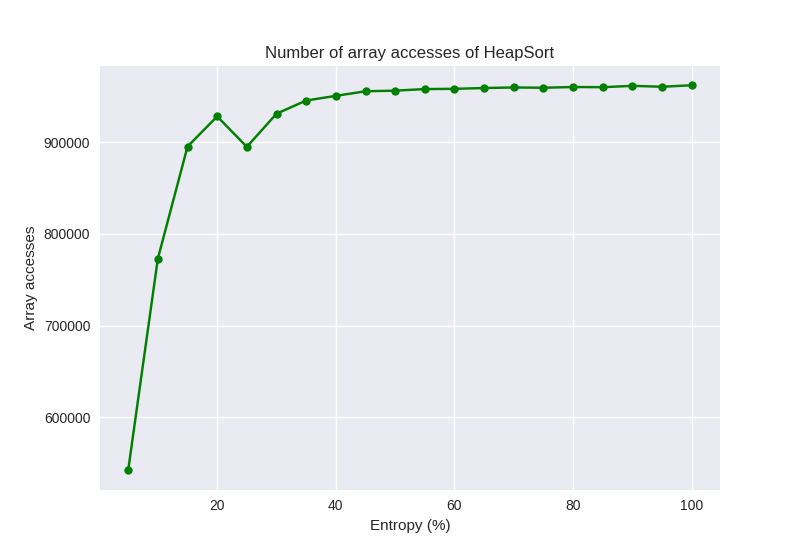
\includegraphics[width=1\textwidth]{graphique/HeapSort/GraphAccessesHeapSort.png}
                \caption{Graphique accès HeapSort}
                \label{fig:mesh1}
            \end{figure}
            \begin{figure}
                \centering
                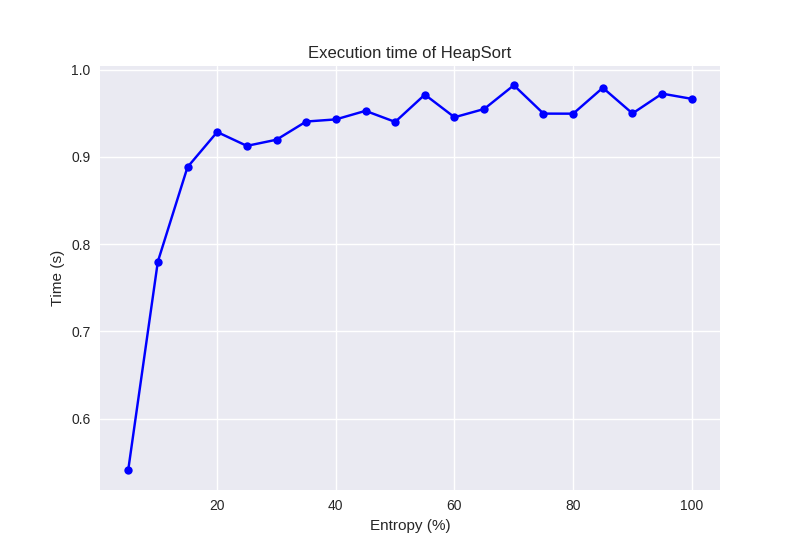
\includegraphics[width=1\textwidth]{graphique/HeapSort/GraphTimeHeapSort.png}
                \caption{Graphique temps HeapSort}
                \label{fig:mesh1}
            \end{figure}
            \begin{figure}
                \centering
                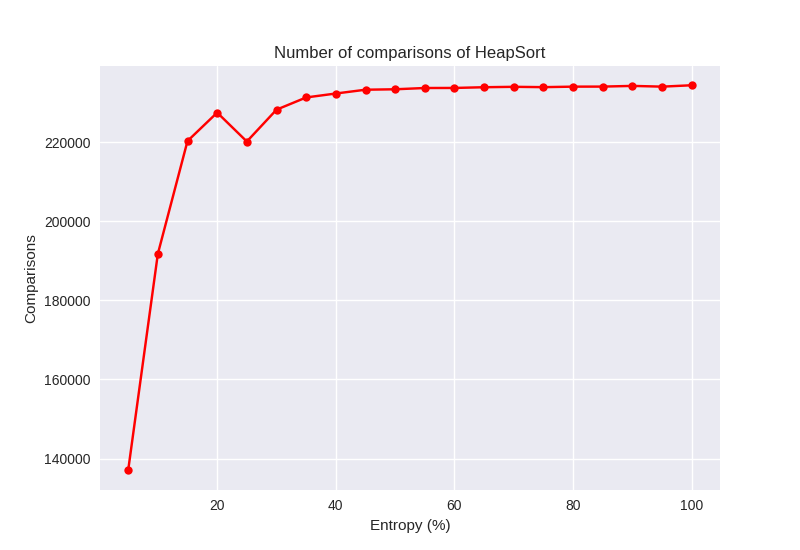
\includegraphics[width=1\textwidth]{graphique/HeapSort/GraphComparisonsHeapSort.png}
                \caption{Graphique comparaisons HeapSort}
                \label{fig:mesh1}
            \end{figure}

%_________________________________________________
            \begin{figure}
                \centering
                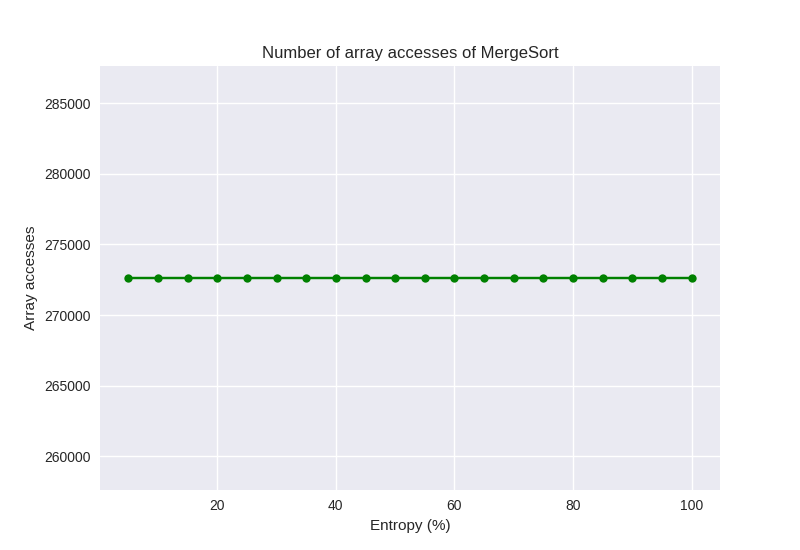
\includegraphics[width=1\textwidth]{graphique/MergeSort/GraphAccessesMergeSort.png}
                \caption{Graphique accès MergeSort}
                \label{fig:mesh1}
            \end{figure}
            \begin{figure}
                \centering
                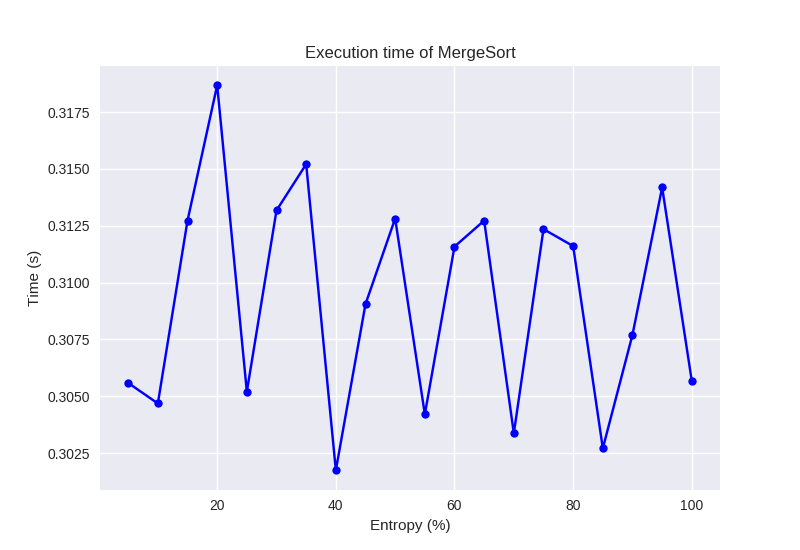
\includegraphics[width=1\textwidth]{graphique/MergeSort/GraphTimeMergeSort.png}
                \caption{Graphique temps MergeSort}
                \label{fig:mesh1}
            \end{figure}
            \begin{figure}
                \centering
                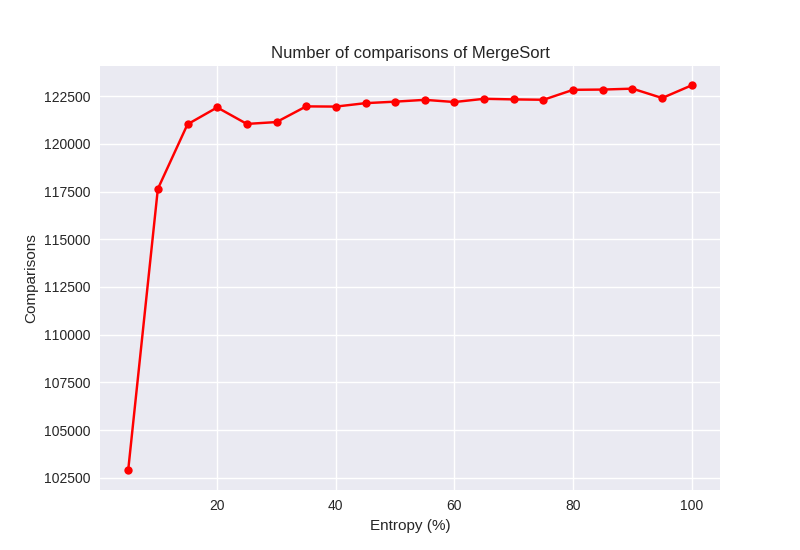
\includegraphics[width=1\textwidth]{graphique/MergeSort/GraphComparisonsMergeSort.png}
                \caption{Graphique comparaisons MergeSort}
                \label{fig:mesh1}
            \end{figure}

%_________________________________________________
            \begin{figure}
                \centering
                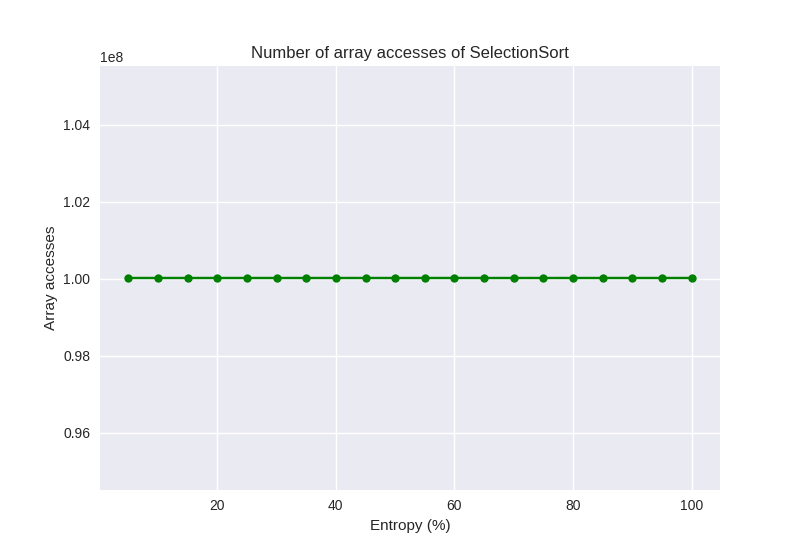
\includegraphics[width=1\textwidth]{graphique/SelectionSort/GraphAccessesSelectionSort.png}
                \caption{Graphique accès SelectionSort}
                \label{fig:mesh1}
            \end{figure}
            \begin{figure}
                \centering
                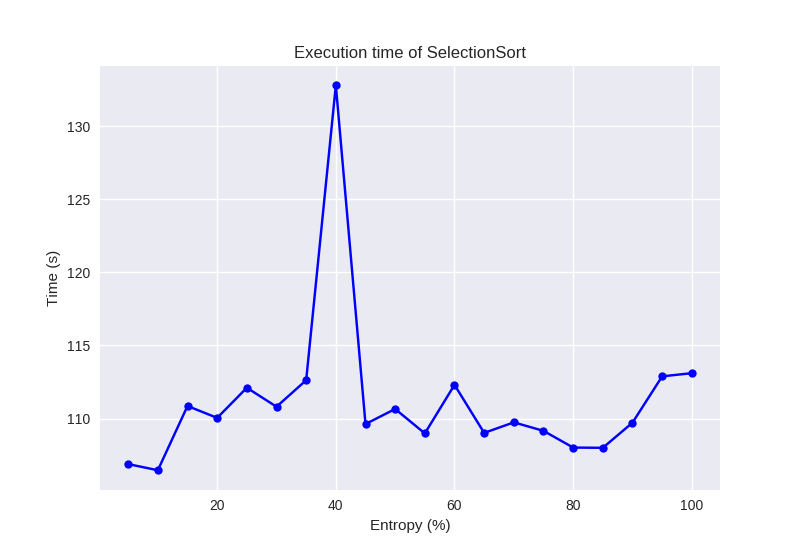
\includegraphics[width=1\textwidth]{graphique/SelectionSort/GraphTimeSelectionSort.png}
                \caption{Graphique temps SelectionSort}
                \label{fig:mesh1}
            \end{figure}
            \begin{figure}
                \centering
                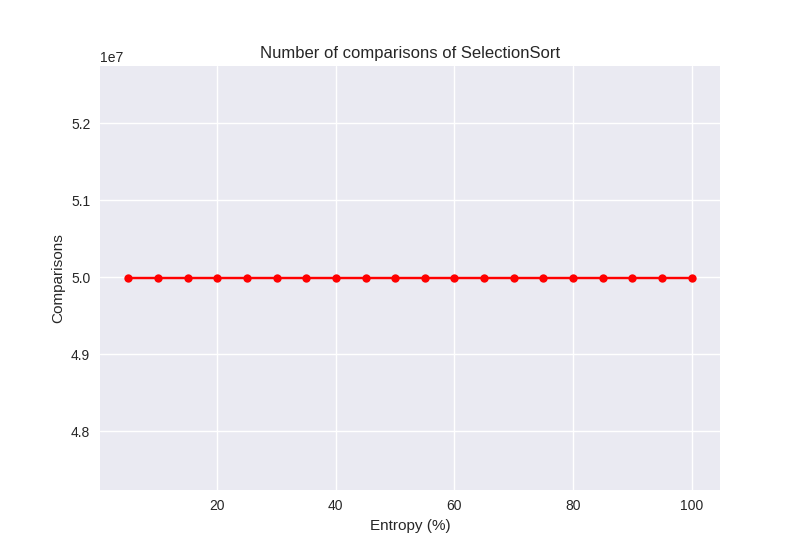
\includegraphics[width=1\textwidth]{graphique/SelectionSort/GraphComparisonsSelectionSort.png}
                \caption{Graphique comparaisons SelectionSort}
                \label{fig:mesh1}
            \end{figure}

%_________________________________________________
            \begin{figure}
                \centering
                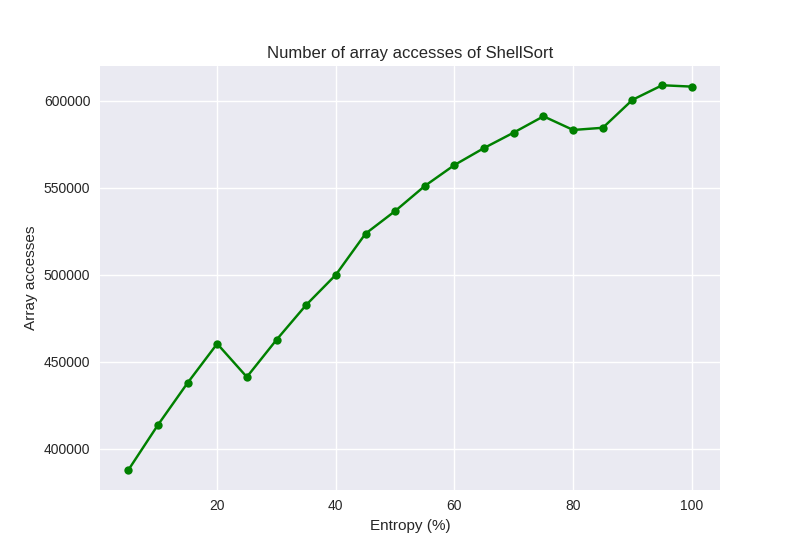
\includegraphics[width=1\textwidth]{graphique/ShellSort/GraphAccessesShellSort.png}
                \caption{Graphique accès ShellSort}
                \label{fig:mesh1}
            \end{figure}
            \begin{figure}
                \centering
                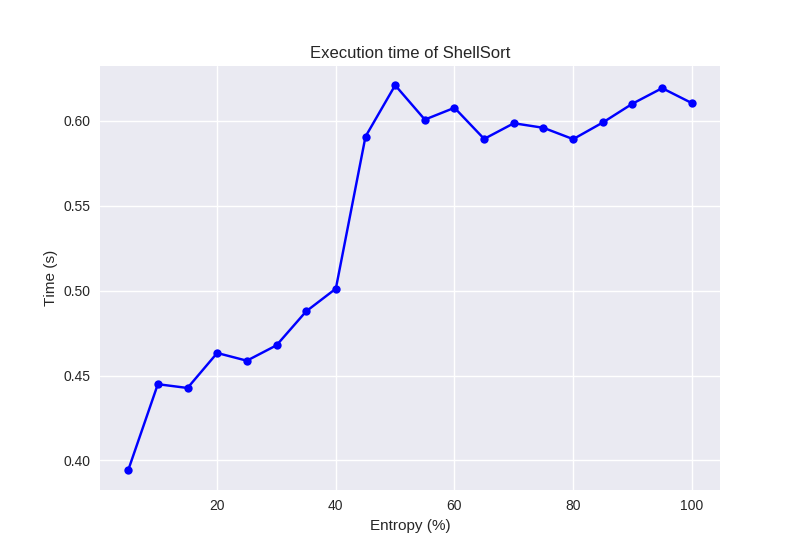
\includegraphics[width=1\textwidth]{graphique/ShellSort/GraphTimeShellSort.png}
                \caption{Graphique temps ShellSort}
                \label{fig:mesh1}
            \end{figure}
            \begin{figure}
                \centering
                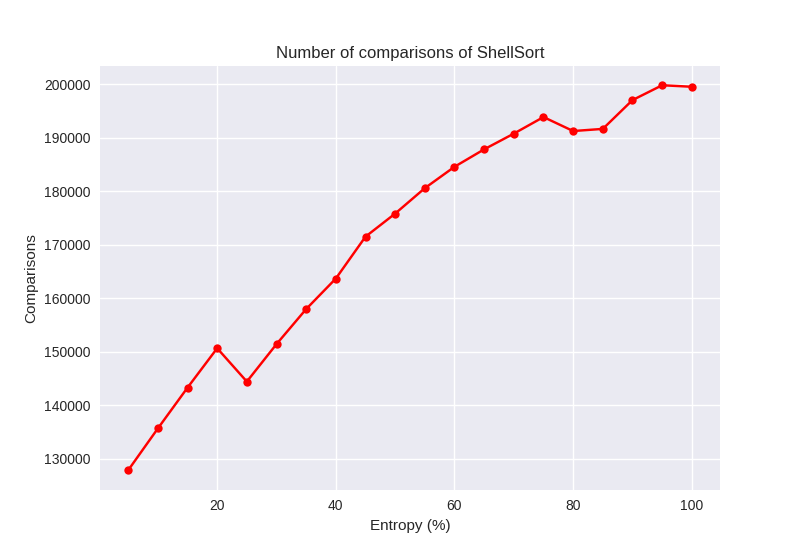
\includegraphics[width=1\textwidth]{graphique/ShellSort/GraphComparisonsShellSort.png}
                \caption{Graphique comparaisons ShellSort}
                \label{fig:mesh1}
            \end{figure}

%_________________________________________________
            \begin{figure}
                \centering
                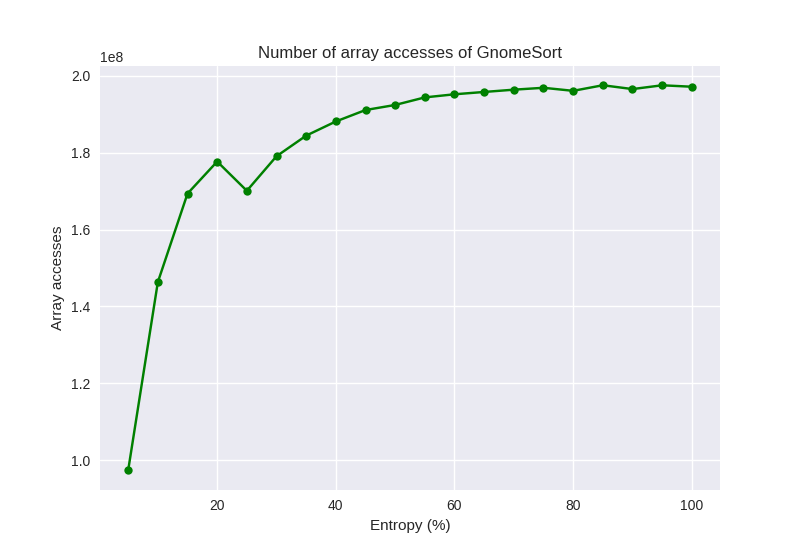
\includegraphics[width=1\textwidth]{graphique/GnomeSort/GraphAccessesGnomeSort.png}
                \caption{Graphique accès GnomeSort}
                \label{fig:mesh1}
            \end{figure}
            \begin{figure}
                \centering
                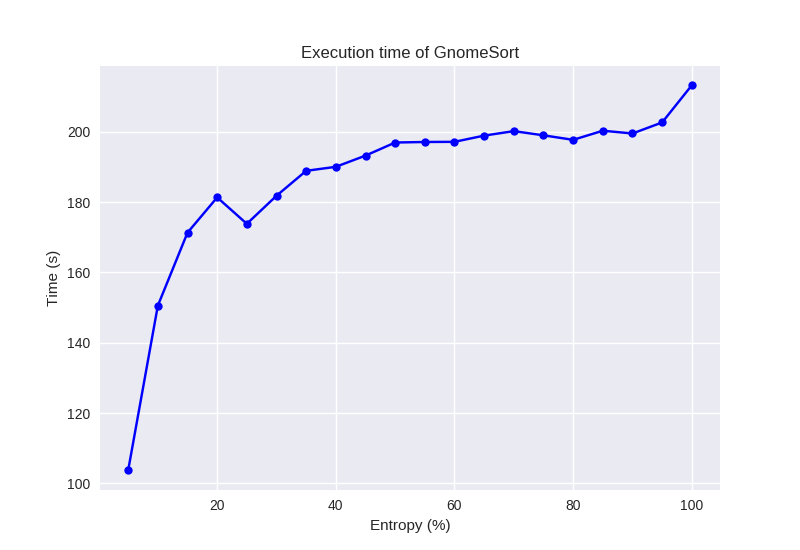
\includegraphics[width=1\textwidth]{graphique/GnomeSort/GraphTimeGnomeSort.png}
                \caption{Graphique temps GnomeSort}
                \label{fig:mesh1}
            \end{figure}
            \begin{figure}
                \centering
                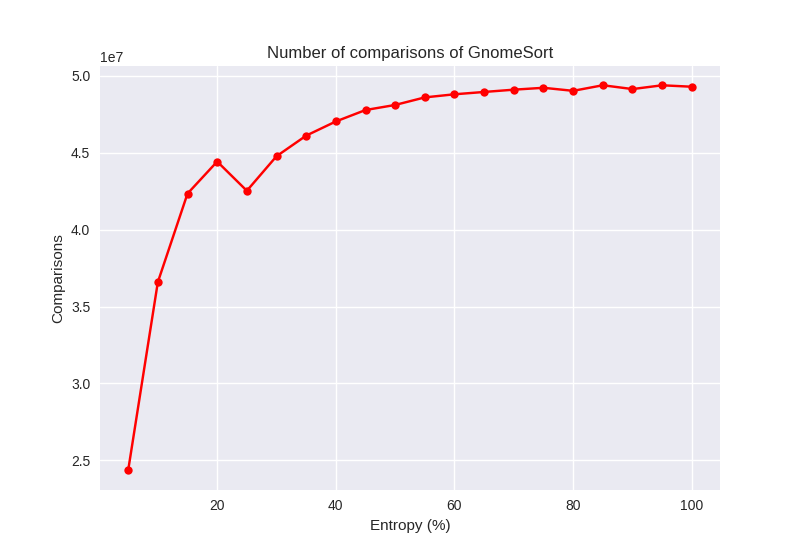
\includegraphics[width=1\textwidth]{graphique/GnomeSort/GraphComparisonsGnomeSort.png}
                \caption{Graphique comparaisons GnomeSort}
                \label{fig:mesh1}
            \end{figure}

%_________________________________________________
            \begin{figure}
                \centering
                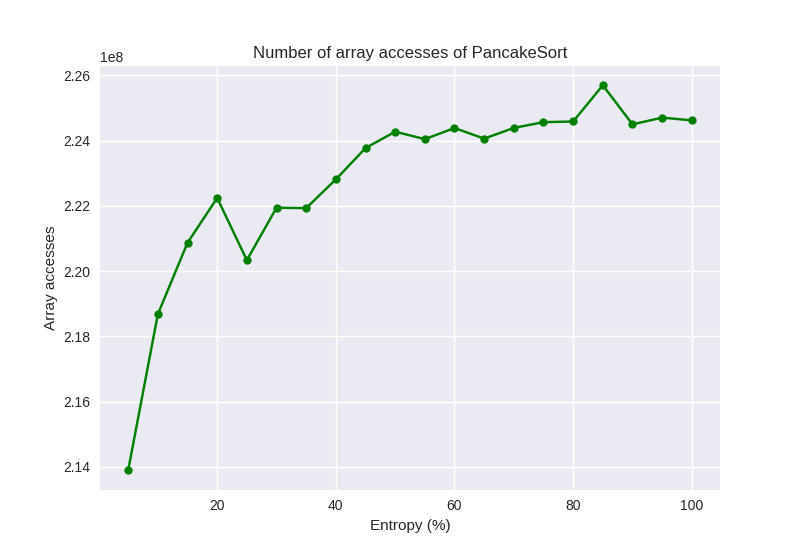
\includegraphics[width=1\textwidth]{graphique/PancakeSort/GraphAccessesPancakeSort.png}
                \caption{Graphique accès PancakeSort}
                \label{fig:mesh1}
            \end{figure}
            \begin{figure}
                \centering
                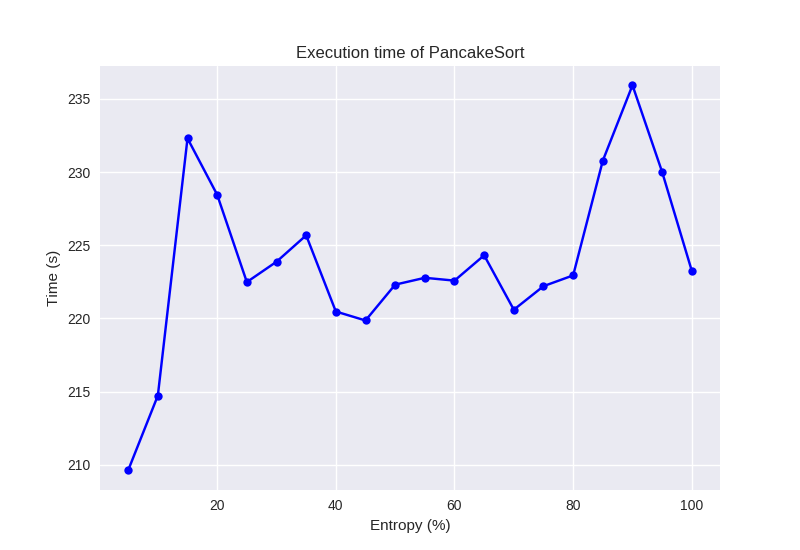
\includegraphics[width=1\textwidth]{graphique/PancakeSort/GraphTimePancakeSort.png}
                \caption{Graphique temps PancakeSort}
                \label{fig:mesh1}
            \end{figure}
            \begin{figure}
                \centering
                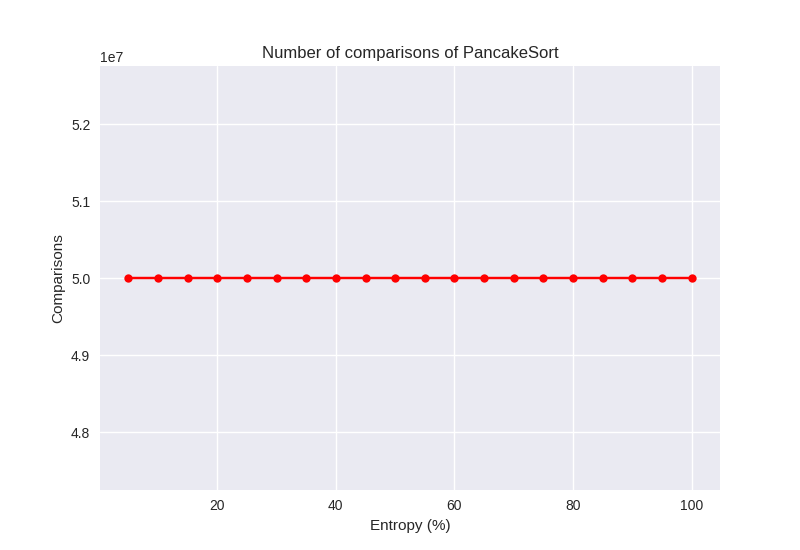
\includegraphics[width=1\textwidth]{graphique/PancakeSort/GraphComparisonsPancakeSort.png}
                \caption{Graphique comparaisons PancakeSort}
                \label{fig:mesh1}
            \end{figure}
\end{document}
